\begin{figure*}[t]
    \centering
    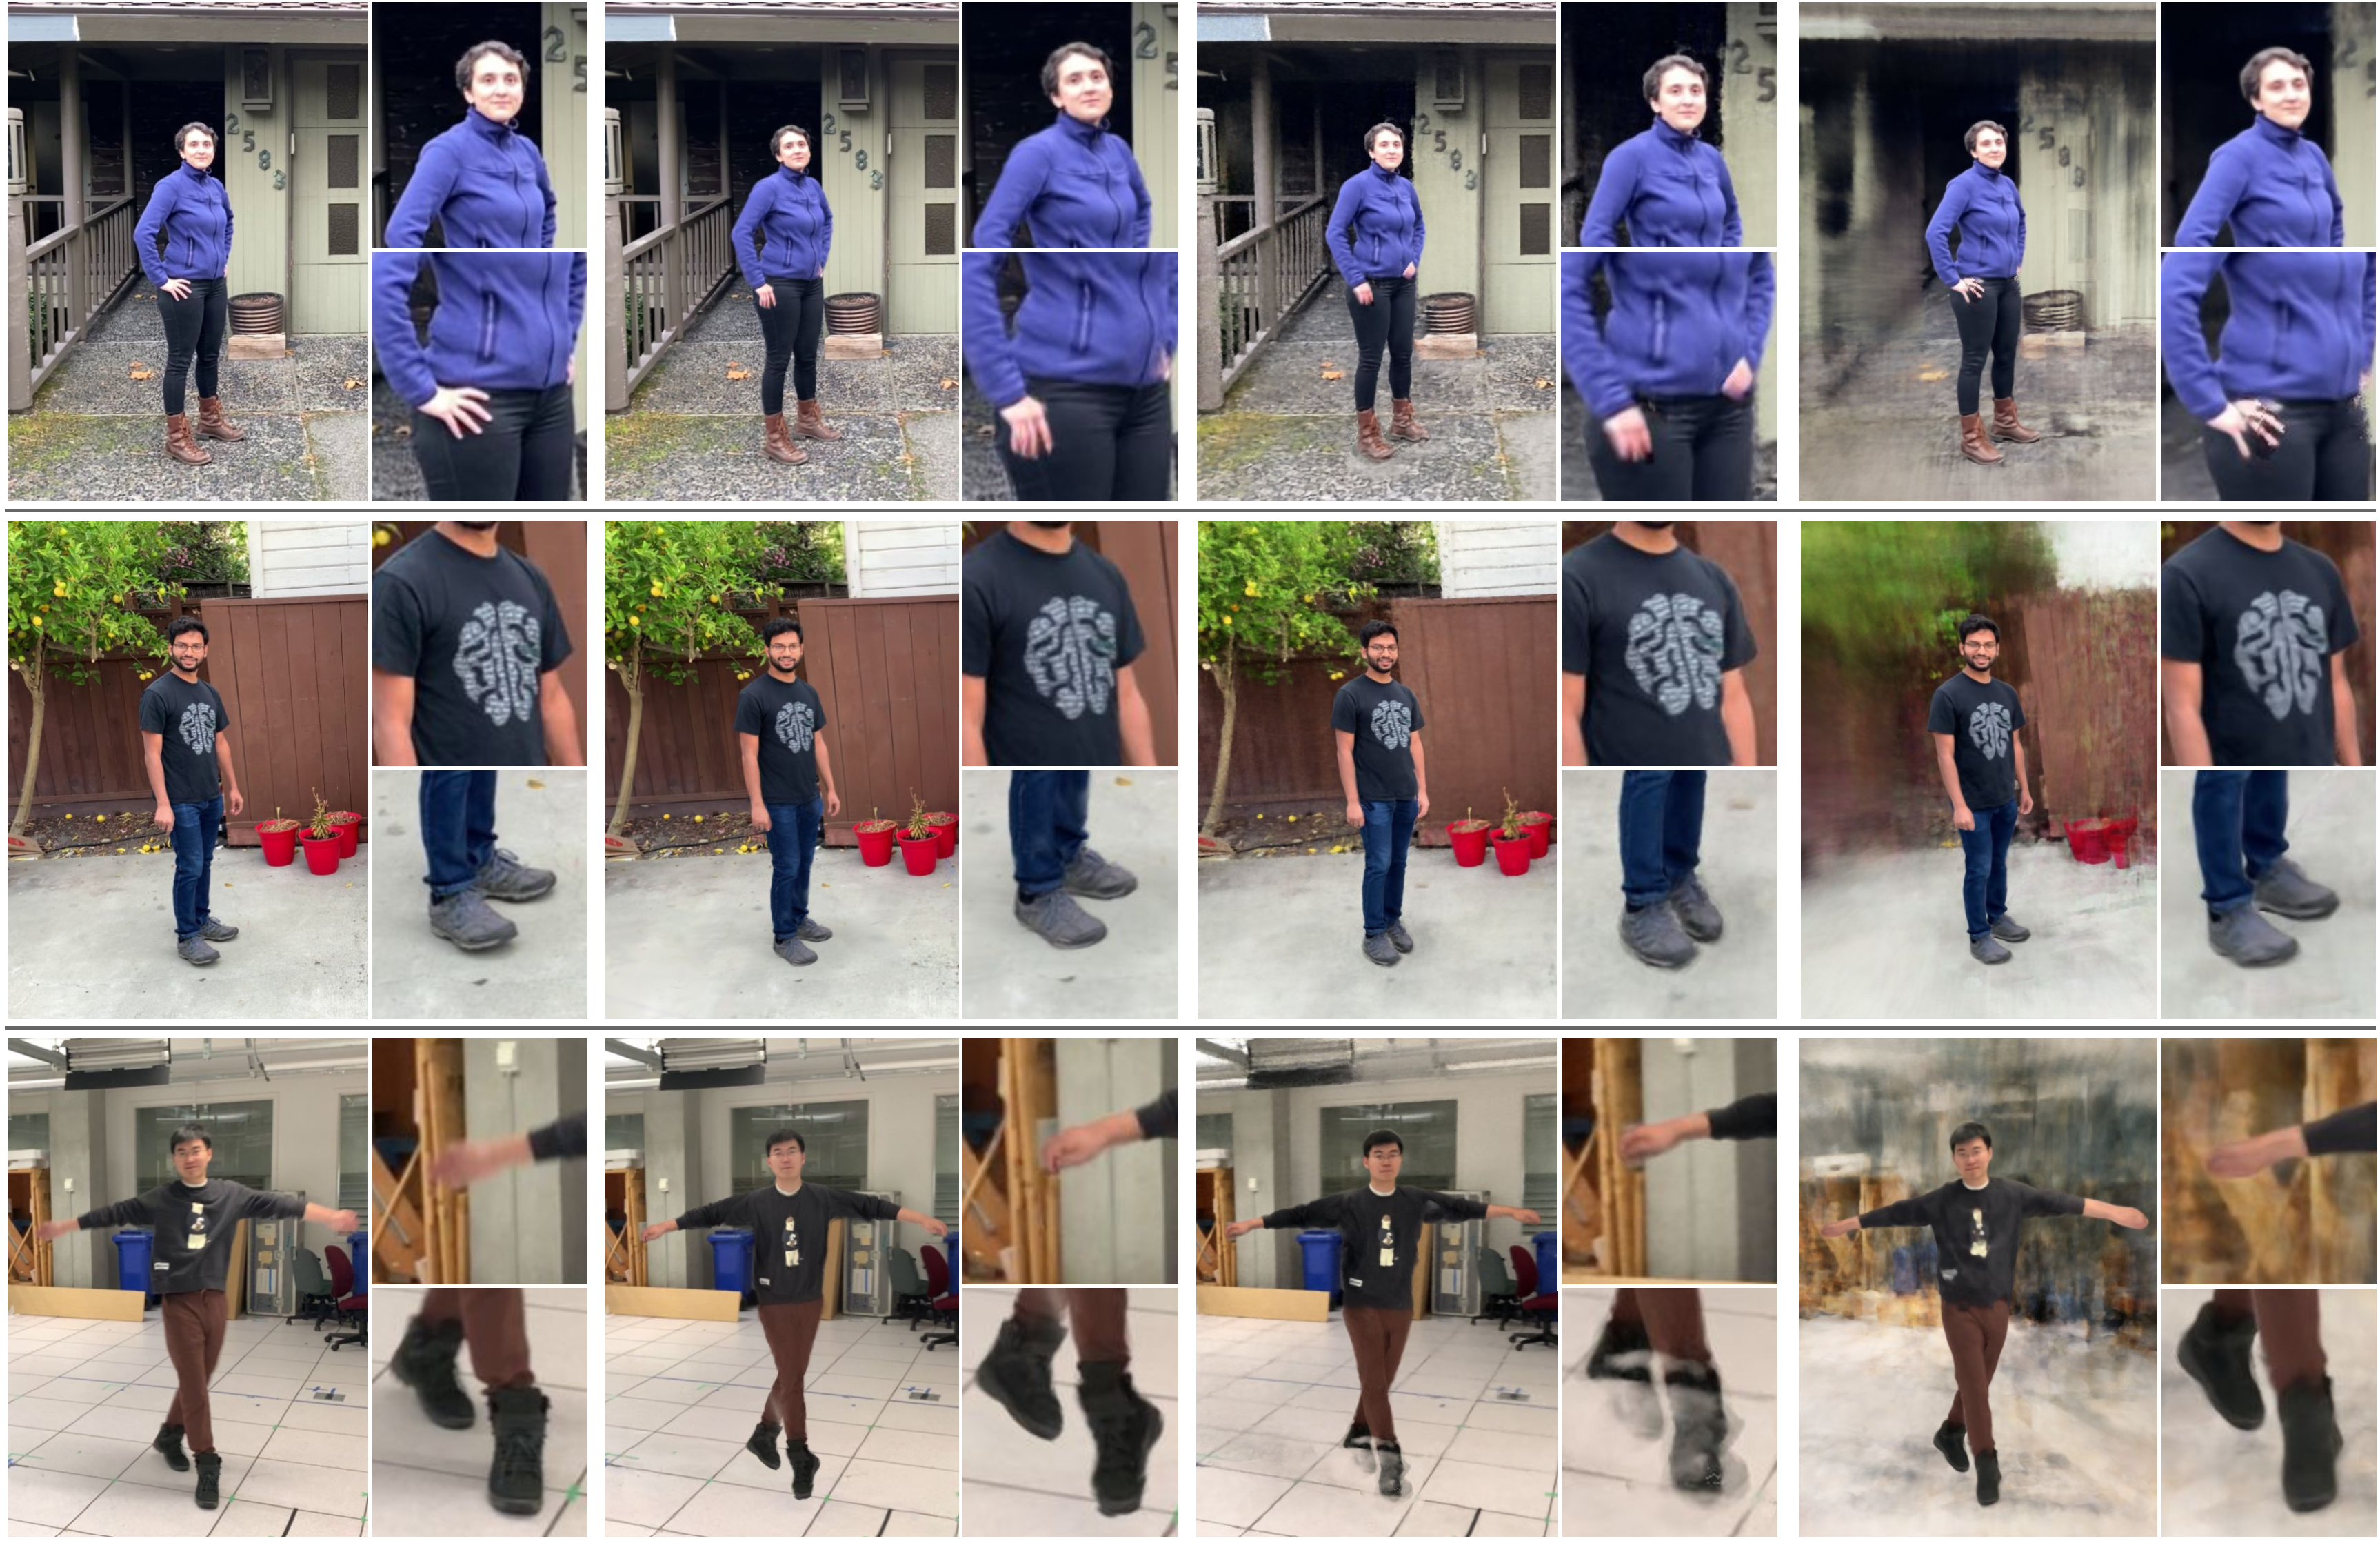
\includegraphics[width=\linewidth]{figures/pdf_files/sota_qual.pdf}
    \small
    \begin{tabular}{cccc}
         \quad Ground Truth \qquad \qquad & \qquad \qquad HUGS (ours) \qquad \qquad & \qquad \quad \qquad NeuMan~\cite{jiang2022neuman} \qquad \quad & \qquad \quad \qquad Vid2Avatar~\cite{guo2023vid2avatar} \qquad 
    \end{tabular}
    \vspace{-3mm}
    \caption{Qualitative results comparing HUGS (ours) with NeuMan and Vid2Avatar with full human (left) and zoomed-in regions (right) for each of the methods. HUGS shows better reconstruction quality especially around hands, feet and clothing wrinkles.} 
    \label{fig:qualitative_sota}
\end{figure*}{}
\begin{figure*}
    \centering
    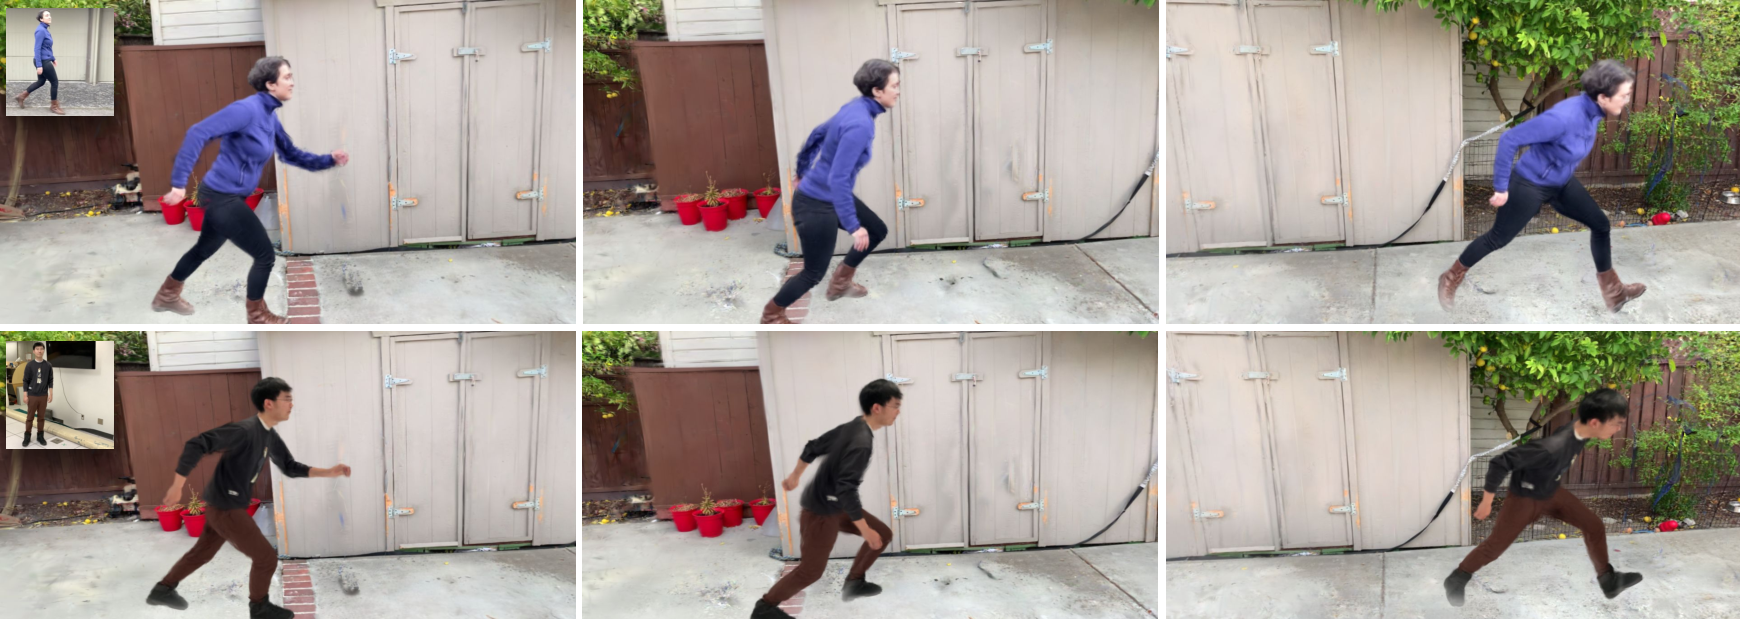
\includegraphics[width=\linewidth]{figures/pdf_files/novel_pose_scene.pdf}
    \caption{Rendering obtained by transferring the Human Gaussians to a different scene. Top-left corner shows the original scene in which the human was captured.}
    \label{fig:composition}
\end{figure*}{}

\section{Experiments}
% \subsection{Implementation details}
\subsection{Datasets}
% \paragraph{NeuMan} We use NeuMan dataset, a collection of 6 videos about 10 to 20 seconds long each, with a single person captured using a mobile phone. Moreover, the camera reasonably pans through the scene to enable multi-view reconstruction. The sequences are named – Seattle, Citron, Parking, Bike, Jogging and Lab. Following the ~\cite{jiang2022neuman} we split frames into 80\% training frames, 10\% validation frames, and 10\% test frames.

% \paragraph{ZJU-MoCap} We evaluate our method on the ZJU-MoCap dataset~\cite{zjumocap} For ZJU-MoCap, following \cite{weng2022humannerf} we select 6 subjects (377, 386, 387, 392, 393, 394) with diverse motions and use images captured by "camera 1" as input and the other 22 cameras for evaluation. We directly apply camera matrices, body pose, and segmentation provided by the dataset.
\paragraph{NeuMan Dataset~\cite{jiang2022neuman}} consists of six videos, each lasting between 10 to 20 seconds, featuring a single individual captured using a mobile phone. The camera pans through the scenes, facilitating multi-view reconstruction. The sequences are denoted as Seattle, Citron, Parking, Bike, Jogging, and Lab. Following the approach outlined in~\cite{jiang2022neuman}, we split frames into 80\% training frames, 10\% validation frames, and 10\% test frames.

\paragraph{ZJU-MoCap Dataset~\cite{peng2021neuralbody}} consists of videos of a human captured in a lab using multi-view capture setup. To align with the methodology in~\cite{weng2022humannerf,yu2023monohuman}, we select six subjects (377, 386, 387, 392, 393, 394) showcasing diverse motions. We employed images captured by "camera 1" as input and utilized the other 22 cameras for evaluation. The camera matrices, body pose, and segmentation provided by the dataset were directly applied in our evaluation process.

\subsection{Qualitative Results}
\label{sec:qualitative}
\paragraph{State-of-the-art Comparison.} We show the qualitative results of our method in ~\cref{fig:qualitative_sota} and compare it with Vid2Avatar~\cite{guo2023vid2avatar} and NeuMan~\cite{jiang2022neuman}. The results are shown from the test samples of the NeuMan dataset~\cite{jiang2022neuman} that are not seen during training.
In the scene background regions, HUGS shows better reconstruction quality than both Vid2Avatar and NeuMan. Vid2Avatar shows blurry scene reconstruction with several artifacts. In contrast, NeuMan shows better scene reconstruction quality but misses fine details such as the house numbers (zoomed-in) in the first row, the wooden plank (zoomed-in) in the second row and the cupboard (zoomed-in) in the third row. In comparison, HUGS shows better reconstruction quality and preserves these fine details as shown in the zoomed-in regions.

In the human regions, Vid2Avatar shows artifacts in the hand region (row 1) and blurry reconstruction in the feet (row 2) and arm region (row 3). In contrast, NeuMan gets better details of the feet regions in some cases (row 2) and introduces artifacts in hands (row 2) and feet (row 3) regions in other cases. In comparison, our method preserves the details around hand and feet and shows better reconstruction quality. Furthermore, our method also preserves the structure around clothing (row 1) where the wrinkles are reconstructed well while preserving the structure of the zipper (zoomed-in) around it compared to previous work.

In summary, we note that HUGS shows better reconstruction quality of both the scene and the human as compared to previous methods while being orders of magnitude faster to train and render (see \S \ref{sec:timing} for speed comparison). We will provide additional qualitative results with videos in the Supp. Mat.

\begin{figure}[t]
    \centering
    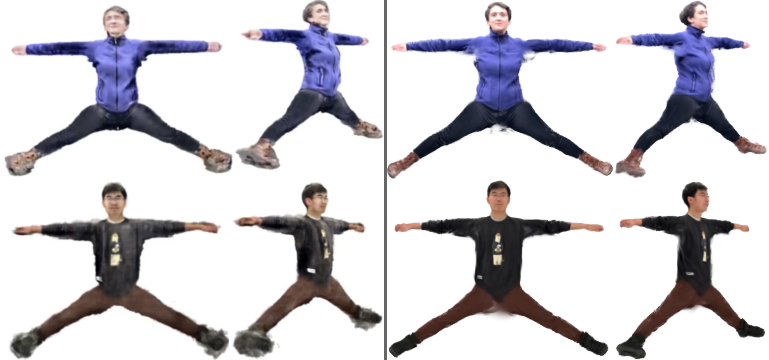
\includegraphics[width=\linewidth]{figures/pdf_files/neuman_canonical.pdf}
    \begin{tabular}{cc}
         NeuMan~\cite{jiang2022neuman} \quad \quad & \qquad \qquad HUGS (ours) 
    \end{tabular}
    \caption{Visualization of Human in canonical Da-pose for HUGS (ours) showing qualitative improvements over NeuMan~\cite{jiang2022neuman}.} 
    \label{fig:canonical}
\end{figure}
\paragraph{Canonical Human Shapes.} In ~\cref{fig:canonical}, we show the reconstruction of the human in the canonical space. We note that our method captures fine details around the feet and hands of the human which look noisy in the case of NeuMan~\cite{jiang2022neuman}. Furthermore, we note that our method preserves rich details on the face. This enables us to achieve high reconstruction quality during the animation phase. 

\definecolor{tabfirst}{rgb}{1, 0.7, 0.7}
\definecolor{tabsecond}{rgb}{1, 0.85, 0.7}
\definecolor{tabthird}{rgb}{1, 1, 0.7}

\begin{table*}[]
    \centering
    \resizebox{\textwidth}{!}{
    \begin{tabular}{c|ccc|ccc|ccc|ccc|ccc|ccc}
    \toprule
        & \multicolumn{3}{c|}{\textbf{Seattle}} & \multicolumn{3}{c|}{\textbf{Citron}} & \multicolumn{3}{c|}{\textbf{Parking}} & \multicolumn{3}{c|}{\textbf{Bike}} & \multicolumn{3}{c|}{\textbf{Jogging}} & \multicolumn{3}{c}{\textbf{Lab}}   \\
    \midrule
        & PSNR $\uparrow$ & SSIM $\uparrow$ & LPIPS $\downarrow$ & PSNR $\uparrow$ & SSIM $\uparrow$ & LPIPS $\downarrow$ & PSNR $\uparrow$ & SSIM $\uparrow$ & LPIPS $\downarrow$ & PSNR $\uparrow$ & SSIM $\uparrow$ & LPIPS $\downarrow$ & PSNR $\uparrow$ & SSIM $\uparrow$ & LPIPS $\downarrow$ & PSNR $\uparrow$ & SSIM $\uparrow$ & LPIPS $\downarrow$  \\
    \midrule
    NeRF-T &        21.84       &      0.69              &       0.37           &               12.33  &          0.49            &        0.65             &       21.98            &             0.69        &        0.46    &   21.16     &      0.71         &     0.36         &     20.63        &       0.53         &         0.49        &     20.52         &    0.75      &       0.39                \\
    % \midrule
    HyperNeRF &    16.43            &     0.43         &    0.40            &     16.81            &    0.41        &          0.56        &      16.04           &           0.38      &         0.62    &     17.64     &   0.42   &      0.43  &       18.52          &  0.39    & 0.52               &      16.75      &    0.51      &     0.23       \\

    
    % \midrule
    Vid2Avatar &  \cellcolor{tabthird}17.41 &  \cellcolor{tabthird}0.56 &  \cellcolor{tabthird}0.60 &  \cellcolor{tabthird}14.32 &  \cellcolor{tabthird}0.62 &  \cellcolor{tabthird}0.65 &  \cellcolor{tabthird}21.56 &  \cellcolor{tabthird}0.69 &  \cellcolor{tabthird}0.50 &  \cellcolor{tabthird}14.86 &  \cellcolor{tabthird}0.51 &  \cellcolor{tabthird}0.69 &  \cellcolor{tabthird}15.04 &  \cellcolor{tabthird}0.41 &  \cellcolor{tabthird}0.70 &  \cellcolor{tabthird}13.96 &  \cellcolor{tabthird}0.60 &  \cellcolor{tabthird}0.68 \\
    % \midrule
    NeuMan     & \cellcolor{tabsecond}23.99 & \cellcolor{tabsecond}0.78 & \cellcolor{tabsecond}0.26 & \cellcolor{tabsecond}24.63 & \cellcolor{tabsecond}0.81 & \cellcolor{tabsecond}0.26 & \cellcolor{tabsecond}25.43 & \cellcolor{tabsecond}0.80 & \cellcolor{tabsecond}0.31 &  \cellcolor{tabfirst}25.55 & \cellcolor{tabsecond}0.83 & \cellcolor{tabsecond}0.23 & \cellcolor{tabsecond}22.70 & \cellcolor{tabsecond}0.68 & \cellcolor{tabsecond}0.32 & \cellcolor{tabsecond}24.96 & \cellcolor{tabsecond}0.86 & \cellcolor{tabsecond}0.21 \\
    \midrule
    HUGS       &  \cellcolor{tabfirst}25.94 &  \cellcolor{tabfirst}0.85 &  \cellcolor{tabfirst}0.13 &  \cellcolor{tabfirst}25.54 &  \cellcolor{tabfirst}0.86 &  \cellcolor{tabfirst}0.15 &  \cellcolor{tabfirst}26.86 &  \cellcolor{tabfirst}0.85 &  \cellcolor{tabfirst}0.22 & \cellcolor{tabsecond}25.46 &  \cellcolor{tabfirst}0.84 &  \cellcolor{tabfirst}0.13 &  \cellcolor{tabfirst}23.75 &  \cellcolor{tabfirst}0.78 &  \cellcolor{tabfirst}0.22 &  \cellcolor{tabfirst}26.00 &  \cellcolor{tabfirst}0.92 &  \cellcolor{tabfirst}0.09
    \\
    \bottomrule
    \end{tabular}  
    }
    \caption{Comparison of HUGS (ours) with previous work on test images of the NeuMan dataset~\cite{jiang2022neuman} using PSNR, SSIM and LPIPS metrics. HUGS achieves state-of-the-art performance across every category with the exception of PSNR on the \textit{Bike} sequence.}
    \label{tab:neuman_human_scene}
\end{table*}
\definecolor{tabfirst}{rgb}{1, 0.7, 0.7}
\definecolor{tabsecond}{rgb}{1, 0.85, 0.7}
\definecolor{tabthird}{rgb}{1, 1, 0.7}

\begin{table*}[htb!]
    \centering
    \resizebox{\textwidth}{!}{
    \begin{tabular}{c|ccc|ccc|ccc|ccc|ccc|ccc}
    \toprule
        & \multicolumn{3}{c|}{\textbf{Seattle}} & \multicolumn{3}{c|}{\textbf{Citron}} & \multicolumn{3}{c|}{\textbf{Parking}} & \multicolumn{3}{c|}{\textbf{Bike}} & \multicolumn{3}{c|}{\textbf{Jogging}} & \multicolumn{3}{c}{\textbf{Lab}}   \\
    \midrule
        & PSNR $\uparrow$ & SSIM $\uparrow$ & LPIPS $\downarrow$ & PSNR $\uparrow$ & SSIM $\uparrow$ & LPIPS $\downarrow$ & PSNR $\uparrow$ & SSIM $\uparrow$ & LPIPS $\downarrow$ & PSNR $\uparrow$ & SSIM $\uparrow$ & LPIPS $\downarrow$ & PSNR $\uparrow$ & SSIM $\uparrow$ & LPIPS $\downarrow$ & PSNR $\uparrow$ & SSIM $\uparrow$ & LPIPS $\downarrow$ \\
    \midrule 
    Vid2Avatar &  \cellcolor{tabthird}16.90 &  \cellcolor{tabthird}0.51 &  \cellcolor{tabthird}0.27 &  \cellcolor{tabthird}15.96 &  \cellcolor{tabthird}0.59 &  \cellcolor{tabthird}0.28 & \cellcolor{tabsecond}18.51 &  \cellcolor{tabthird}0.65 &  \cellcolor{tabthird}0.26 &  \cellcolor{tabthird}12.44 &  \cellcolor{tabthird}0.39 &  \cellcolor{tabthird}0.54 &  \cellcolor{tabthird}16.36 &  \cellcolor{tabthird}0.46 &  \cellcolor{tabthird}0.30 &  \cellcolor{tabthird}15.99 &  \cellcolor{tabthird}0.62 &  \cellcolor{tabthird}0.34 \\
    % \midrule
    NeuMan     & \cellcolor{tabsecond}18.42 & \cellcolor{tabsecond}0.58 & \cellcolor{tabsecond}0.20 & \cellcolor{tabsecond}18.39 & \cellcolor{tabsecond}0.64 & \cellcolor{tabsecond}0.19 &  \cellcolor{tabthird}17.66 & \cellcolor{tabsecond}0.66 & \cellcolor{tabsecond}0.24 & \cellcolor{tabsecond}19.05 & \cellcolor{tabsecond}0.66 & \cellcolor{tabsecond}0.21 &  \cellcolor{tabfirst}17.57 & \cellcolor{tabsecond}0.54 & \cellcolor{tabsecond}0.29 & \cellcolor{tabsecond}18.76 & \cellcolor{tabsecond}0.73 & \cellcolor{tabsecond}0.23 \\
    \midrule
    HUGS       &  \cellcolor{tabfirst}19.06 &  \cellcolor{tabfirst}0.67 &  \cellcolor{tabfirst}0.15 &  \cellcolor{tabfirst}19.16 &  \cellcolor{tabfirst}0.71 &  \cellcolor{tabfirst}0.16 &  \cellcolor{tabfirst}19.44 &  \cellcolor{tabfirst}0.73 &  \cellcolor{tabfirst}0.17 &  \cellcolor{tabfirst}19.48 &  \cellcolor{tabfirst}0.67 &  \cellcolor{tabfirst}0.18 & \cellcolor{tabsecond}17.45 &  \cellcolor{tabfirst}0.59 &  \cellcolor{tabfirst}0.27 &  \cellcolor{tabfirst}18.79 &  \cellcolor{tabfirst}0.76 &  \cellcolor{tabfirst}0.18
    
\\
    \bottomrule
    \end{tabular}  
    }
    \caption{Comparison of HUGS (ours) with previous work on the NeuMan dataset~\cite{jiang2022neuman} over \textbf{human-only} regions cropped using a tight bounding box. Performance is evaluated on PSNR, SSIM and LPIPS metrics.}
    \label{tab:neuman_human}
\end{table*}
\definecolor{tabfirst}{rgb}{1, 0.7, 0.7}
\definecolor{tabsecond}{rgb}{1, 0.85, 0.7}
\definecolor{tabthird}{rgb}{1, 1, 0.7}

\begin{table*}[htb!]
    \centering
    \resizebox{\textwidth}{!}{
    \begin{tabular}{c|ccc|ccc|ccc|ccc|ccc|ccc}
    \toprule
        & \multicolumn{3}{c|}{\textbf{377}} & \multicolumn{3}{c|}{\textbf{386}} & \multicolumn{3}{c|}{\textbf{387}} & \multicolumn{3}{c|}{\textbf{392}} & \multicolumn{3}{c|}{\textbf{393}} & \multicolumn{3}{c}{\textbf{394}}   \\
    \midrule
        & PSNR $\uparrow$ & SSIM $\uparrow$ & LPIPS $\downarrow$ & PSNR $\uparrow$ & SSIM $\uparrow$ & LPIPS $\downarrow$ & PSNR $\uparrow$ & SSIM $\uparrow$ & LPIPS $\downarrow$ & PSNR $\uparrow$ & SSIM $\uparrow$ & LPIPS $\downarrow$ & PSNR $\uparrow$ & SSIM $\uparrow$ & LPIPS $\downarrow$ & PSNR $\uparrow$ & SSIM $\uparrow$ & LPIPS $\downarrow$  \\
    \midrule
    %     NeuralBody & 29.11 & 0.97 & 40.95 & 30.54 & 0.97 & 46.43 & 27.00 & 0.95 & 59.47 & 30.10 & 0.96 & 53.27 & 28.61 & 0.96 & 59.05 & 29.10 & 0.96 & 54.55 & 1 days \\
    % \midrule
    %     HumanNerf & 30.41 & 0.97 & 24.06 & 33.20 & 0.98 & 28.99 & 28.18 & 0.96 & 35.58 & 31.04 & 0.97 & 32.12 & 28.31 & 0.96 & 36.72 & 30.31 & 0.96 & \textbf{32.89} & 1 days \\
    % \midrule
    %     MonoHuman & 30.77 & 0.98 & \textbf{21.67} & 32.97 & 0.97 & 32.73 & 27.93 & 0.96 & \textbf{33.45} & 31.24 & 0.97 & \textbf{31.04} & 28.46 & 0.96 & 34.24 & 28.94 & 0.96 & 35.90 & 1 days \\
    % \midrule
    %     HUGS      & \textbf{30.89} & \textbf{0.98} & 26.13 & \textbf{34.00 }& \textbf{0.98} & \textbf{28.78} &\textbf{ 29.41} & \textbf{0.97} & 35.04 & \textbf{31.75} & \textbf{0.98} & 31.32 & \textbf{29.91} & \textbf{0.97} & \textbf{34.70} & \textbf{31.06} & \textbf{ 0.97} & 33.13 & 35 mins \\ 

NeuralBody &                      29.11 & \cellcolor{tabsecond}0.97 & \cellcolor{tabsecond}0.04 &                      30.54 & \cellcolor{tabsecond}0.97 &  \cellcolor{tabthird}0.05 &                      27.00 &  \cellcolor{tabthird}0.95 &  \cellcolor{tabthird}0.06 &                      30.10 & \cellcolor{tabsecond}0.96 & \cellcolor{tabsecond}0.05 & \cellcolor{tabsecond}28.61 & \cellcolor{tabsecond}0.96 &  \cellcolor{tabthird}0.06 &  \cellcolor{tabthird}29.10 & \cellcolor{tabsecond}0.96 &  \cellcolor{tabthird}0.05 \\

HumanNerf  &  \cellcolor{tabthird}30.41 & \cellcolor{tabsecond}0.97 &  \cellcolor{tabfirst}0.02 & \cellcolor{tabsecond}33.20 &  \cellcolor{tabfirst}0.98 & \cellcolor{tabsecond}0.03 & \cellcolor{tabsecond}28.18 & \cellcolor{tabsecond}0.96 & \cellcolor{tabsecond}0.04 &  \cellcolor{tabthird}31.04 &  \cellcolor{tabfirst}0.97 &  \cellcolor{tabfirst}0.03 &                      28.31 & \cellcolor{tabsecond}0.96 & \cellcolor{tabsecond}0.04 & \cellcolor{tabsecond}30.31 & \cellcolor{tabsecond}0.96 &  \cellcolor{tabfirst}0.03  \\
MonoHuman  & \cellcolor{tabsecond}30.77 &  \cellcolor{tabfirst}0.98 &  \cellcolor{tabfirst}0.02 &  \cellcolor{tabthird}32.97 & \cellcolor{tabsecond}0.97 & \cellcolor{tabsecond}0.03 &  \cellcolor{tabthird}27.93 & \cellcolor{tabsecond}0.96 &  \cellcolor{tabfirst}0.03 & \cellcolor{tabsecond}31.24 &  \cellcolor{tabfirst}0.97 &  \cellcolor{tabfirst}0.03 &  \cellcolor{tabthird}28.46 & \cellcolor{tabsecond}0.96 &  \cellcolor{tabfirst}0.03 &                      28.94 & \cellcolor{tabsecond}0.96 & \cellcolor{tabsecond}0.04  \\
\midrule
\acronym   &  \cellcolor{tabfirst}30.80 &  \cellcolor{tabfirst}0.98 &  \cellcolor{tabfirst}0.02 &  \cellcolor{tabfirst}34.11 &  \cellcolor{tabfirst}0.98 &  \cellcolor{tabfirst}0.02 &  \cellcolor{tabfirst}29.29 &  \cellcolor{tabfirst}0.97 &  \cellcolor{tabfirst}0.03 &  \cellcolor{tabfirst}31.36 &  \cellcolor{tabfirst}0.97 &  \cellcolor{tabfirst}0.03 &  \cellcolor{tabfirst}29.80 &  \cellcolor{tabfirst}0.97 &  \cellcolor{tabfirst}0.03 &  \cellcolor{tabfirst}30.54 &  \cellcolor{tabfirst}0.97 &  \cellcolor{tabfirst}0.03  \\

    \bottomrule
    \end{tabular}  
    }
    \caption{Comparison of HUGS (ours) with the previous work on the ZJU Mocap dataset~\cite{peng2021neuralbody}. Performance is evaluated on PSNR, SSIM and LPIPS metric. HUGS achieves state-of-the-art performance across all scenes and all metrics.}
    \label{tab:zju}
\end{table*}



\paragraph{Disentanglement of the Human and the Scene.} HUGS allows for a disentangled represenation of the human and the scene by storing their Gaussian features separately. This allows us to move the human to different scenes. In \cref{fig:composition}, we show the composition of human captured in one scene into a different scene. We show additional video results in the supplemental material.


\subsection{Quantitative Results}
\label{sec:quantitative}
We compare the performance of our method with baselines such as NeRF-T~\cite{li2021neural}, HyperNeRF~\cite{park2021hypernerf} and the existing state-of-the-art methods -- NeuMan~\cite{jiang2022neuman} and Vid2Avatar~\cite{guo2023vid2avatar}.

In \cref{tab:neuman_human_scene}, we evaluate the reconstruction quality on the NeuMan dataset~\cite{jiang2022neuman} on three different metrics -- Peak Signal-to-Noise Ration (PSNR), SSIM~\cite{ssim} and LPIPS~\cite{zhang2018lpips}. NeRF-T and HyperNeRF are general dynamic scene reconstruction methods and do not specialize for humans. Therefore, they show poor reconstruction quality. On the other hand, NeuMan and Vid2Avatar employ specialized models for the human and the scene. NeuMan employs a NeRF-based~\cite{mildenhall2020nerf} approach for both scene and human modeling. Vid2Avatar utilizes an implicit SDF model and volume rendering for scene and human representation. Therefore, both NeuMan and Vid2Avatar show improved reconstruction quality. In comparison, our method achieves state-of-the-art performance across all the scenes and metrics except PSNR on the \textit{Bike} sequence where we show competitive performance.

In \cref{tab:neuman_human}, we further evaluate the reconstruction error but only on the regions containing the human. We first take a tight crop around the human region in the ground truth image. This crop is used over all the predictions, and the reconstruction error is evaluated over the cropped samples. It should be noted that we take rectangular crops of the region and do not use any segmentation mask since reconstruction metrics are highly sensitive to masks. Under this evaluation, we show state-of-the-art performance across all scenes and metrics except PSNR on the \textit{Jogging} sequence where we show competitive performance. 

In addition, we evaluate our method using the ZJU Mocap dataset~\cite{peng2021neuralbody} in ~\cref{tab:zju}. We compare with recent previous work that report their evaluation on this dataset which include NeuralBody~\cite{peng2021neuralbody}, HumanNerf~\cite{weng2022humannerf}, and MonoHuman~\cite{yu2023monohuman}. 

%As these models are all NeRF-based, they share the drawback of being slow in both training and rendering. Notably, our method stands out as both faster and more accurate than the listed state-of-the-art models, providing a compelling combination of efficiency and precision.



%In \cref{tab:neuman_human_scene} \cref{tab:neuman_human}, we present a comparative analysis of our method against existing joint human and scene novel view synthesis approaches. Given the novelty of this task, research in this domain is limited. Notable existing works include NeuMan~\cite{jiang2022neuman} and Vid2Avatar~\cite{guo2023vid2avatar}.

\label{sec:timing}
\begin{figure}[t]
    \centering
    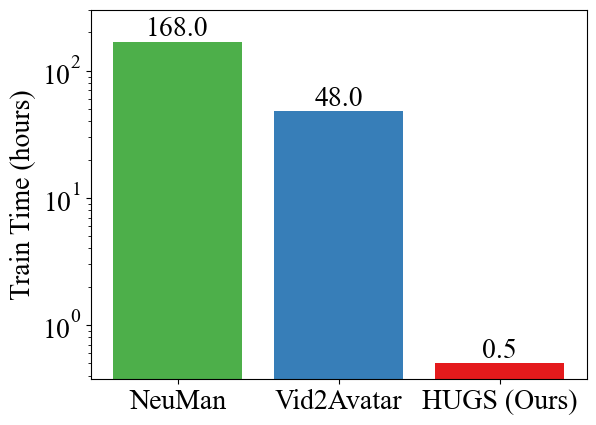
\includegraphics[width=0.49\linewidth]{figures/pngs/train_time.png}
    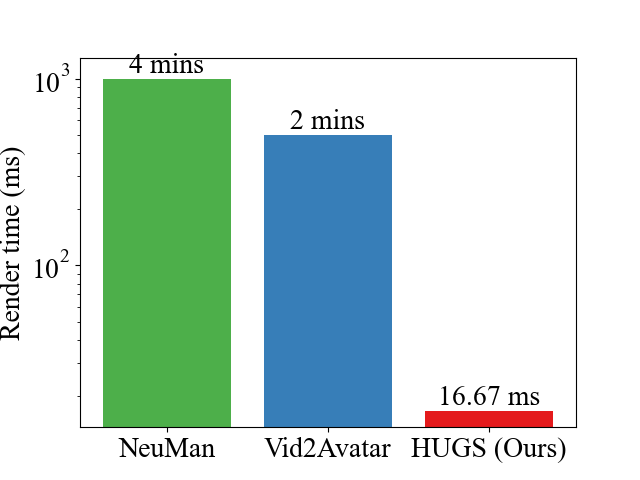
\includegraphics[width=0.49\linewidth]{figures/pngs/render_time.png}
    \caption{{Timing comparison for training in hours and rendering in milliseconds. y-axis is  on log-scale. HUGS outperforms previous methods by an order of magnitude. }} 
    \label{fig:timing}
\end{figure}
\begin{table*}[t]
    \centering
    \resizebox{\textwidth}{!}{
    \begin{tabular}{l|ccc|ccc|ccc|ccc|ccc|ccc}
    \toprule
        & \multicolumn{3}{c|}{\textbf{Seattle}} & \multicolumn{3}{c|}{\textbf{Citron}} & \multicolumn{3}{c|}{\textbf{Parking}} & \multicolumn{3}{c|}{\textbf{Bike}} & \multicolumn{3}{c|}{\textbf{Jogging}} & \multicolumn{3}{c}{\textbf{Lab}}   \\
    \midrule
        & PSNR $\uparrow$ & SSIM $\uparrow$ & LPIPS $\downarrow$ & PSNR $\uparrow$ & SSIM $\uparrow$ & LPIPS $\downarrow$ & PSNR $\uparrow$ & SSIM $\uparrow$ & LPIPS $\downarrow$ & PSNR $\uparrow$ & SSIM $\uparrow$ & LPIPS $\downarrow$ & PSNR $\uparrow$ & SSIM $\uparrow$ & LPIPS $\downarrow$ & PSNR $\uparrow$ & SSIM $\uparrow$ & LPIPS $\downarrow$  \\
    \midrule
    w/o LBS             &                      18.47 & \cellcolor{tabsecond}0.66 & \cellcolor{tabsecond}0.16 & \cellcolor{tabsecond}19.00 & \cellcolor{tabsecond}0.70 &  \cellcolor{tabfirst}0.16 & \cellcolor{tabsecond}19.13 & \cellcolor{tabsecond}0.72 & \cellcolor{tabsecond}0.19 & \cellcolor{tabsecond}19.73 &  \cellcolor{tabfirst}0.68 &  \cellcolor{tabfirst}0.18 &                      17.29 &  \cellcolor{tabthird}0.58 &  \cellcolor{tabthird}0.27 &  \cellcolor{tabthird}18.80 &  \cellcolor{tabfirst}0.76 &  \cellcolor{tabfirst}0.18 \\
    \midrule
    w/o Densify         & \cellcolor{tabsecond}18.91 &  \cellcolor{tabthird}0.65 & \cellcolor{tabsecond}0.16 &                      17.18 &  \cellcolor{tabthird}0.68 &  \cellcolor{tabthird}0.18 &  \cellcolor{tabthird}19.00 &  \cellcolor{tabthird}0.71 &  \cellcolor{tabthird}0.21 &  \cellcolor{tabfirst}19.92 & \cellcolor{tabsecond}0.67 & \cellcolor{tabsecond}0.19 & \cellcolor{tabsecond}17.63 &                      0.57 & \cellcolor{tabsecond}0.26 &  \cellcolor{tabfirst}18.98 &  \cellcolor{tabfirst}0.76 &  \cellcolor{tabfirst}0.18 \\
    \midrule
    w/o $\mathcal{L}^h$ &  \cellcolor{tabthird}18.87 &  \cellcolor{tabfirst}0.67 & \cellcolor{tabsecond}0.16 &  \cellcolor{tabthird}17.31 &                      0.67 &                      0.19 &                      17.76 &                      0.70 &                      0.23 &  \cellcolor{tabthird}19.63 &  \cellcolor{tabfirst}0.68 & \cellcolor{tabsecond}0.19 &  \cellcolor{tabfirst}18.23 &  \cellcolor{tabfirst}0.60 & \cellcolor{tabsecond}0.26 &                      18.75 &  \cellcolor{tabfirst}0.76 & \cellcolor{tabsecond}0.19 \\
    \midrule
    w/o Triplane        &                      18.70 &  \cellcolor{tabthird}0.65 &  \cellcolor{tabfirst}0.15 &                      17.12 &                      0.67 & \cellcolor{tabsecond}0.17 &                      18.78 &                      0.69 & \cellcolor{tabsecond}0.19 &                      19.52 &  \cellcolor{tabthird}0.66 &  \cellcolor{tabfirst}0.18 &  \cellcolor{tabthird}17.60 &                      0.56 &  \cellcolor{tabfirst}0.25 & \cellcolor{tabsecond}18.91 & \cellcolor{tabsecond}0.74 & \cellcolor{tabsecond}0.19 \\
    \midrule
    HUGS                &  \cellcolor{tabfirst}19.06 &  \cellcolor{tabfirst}0.67 &  \cellcolor{tabfirst}0.15 &  \cellcolor{tabfirst}19.16 &  \cellcolor{tabfirst}0.71 &  \cellcolor{tabfirst}0.16 &  \cellcolor{tabfirst}19.44 &  \cellcolor{tabfirst}0.73 &  \cellcolor{tabfirst}0.17 &                      19.48 & \cellcolor{tabsecond}0.67 &  \cellcolor{tabfirst}0.18 &                      17.45 & \cellcolor{tabsecond}0.59 &  \cellcolor{tabthird}0.27 &                      18.79 &  \cellcolor{tabfirst}0.76 &  \cellcolor{tabfirst}0.18
    \\ 
    \bottomrule
    \end{tabular}  
    }
    \caption{\textbf{Ablation study.} The performance is evaluated over human-only bounding box regions using PSNR, SSIM and LPIPS metrics. }
    \label{tab:neuman_ablation_human_only}
\end{table*}

\paragraph{Speed.} In ~\cref{fig:timing}, we compare the training and rendering time of our method with previous work. The use of 3DGS~\cite{kerbl3Dgaussians} speeds up our training and rendering times by a significant margin. We note that HUGS is {$96 \times$} faster than Vid2Avatar and {$336 \times $} faster than NeuMan  training within 30 minutes.
At rendering time, we do not rely on MLPs and only use the LBS weights, enabling higher frame rate.
%
Our method achieves {60 FPS} outperforming NeuMan by {${\sim}7600 \times$} and Vid2Avatar by {${\sim}3800 \times$}. We benchmark all the methods on a single GeForce 3090Ti GPU. \\
%Furthermore, our method enables training within 30 minutes \ar{z times} faster than NeuMan.

%However, NeRF models are characterized by lengthy training and rendering times. Vid2Avatar, on the other hand, utilizes an implicit SDF model and volume rendering for scene and human representation, but this method proves to be prohibitively slow, as indicated by the training and inference time comparison in the tables. In contrast, 

In summary, our model demonstrates efficiency in both training and rendering, delivering superior results compared to existing methods. 
Our model not only outperforms established NeRF and implicit-SDF based models but does so at orders of magnitude faster speeds.


\subsection{Ablation Experiments}
% \begin{table*}[]
    \centering
    \resizebox{\textwidth}{!}{
    \begin{tabular}{l|ccc|ccc|ccc|ccc|ccc|ccc}
    \toprule
        & \multicolumn{3}{c|}{\textbf{Seattle}} & \multicolumn{3}{c|}{\textbf{Citron}} & \multicolumn{3}{c|}{\textbf{Parking}} & \multicolumn{3}{c|}{\textbf{Bike}} & \multicolumn{3}{c|}{\textbf{Jogging}} & \multicolumn{3}{c}{\textbf{Lab}}   \\
    \midrule
        & PSNR $\uparrow$ & SSIM $\uparrow$ & LPIPS $\downarrow$ & PSNR $\uparrow$ & SSIM $\uparrow$ & LPIPS $\downarrow$ & PSNR $\uparrow$ & SSIM $\uparrow$ & LPIPS $\downarrow$ & PSNR $\uparrow$ & SSIM $\uparrow$ & LPIPS $\downarrow$ & PSNR $\uparrow$ & SSIM $\uparrow$ & LPIPS $\downarrow$ & PSNR $\uparrow$ & SSIM $\uparrow$ & LPIPS $\downarrow$  \\
    \midrule
    w/o LBS             &                      25.80 &  \cellcolor{tabfirst}0.85 & \cellcolor{tabsecond}0.14 & \cellcolor{tabsecond}25.36 &  \cellcolor{tabfirst}0.86 &  \cellcolor{tabfirst}0.15 & \cellcolor{tabsecond}26.68 &  \cellcolor{tabfirst}0.85 & \cellcolor{tabsecond}0.23 &  \cellcolor{tabfirst}25.62 & \cellcolor{tabsecond}0.84 &  \cellcolor{tabfirst}0.13 &  \cellcolor{tabthird}23.70 &  \cellcolor{tabfirst}0.78 & \cellcolor{tabsecond}0.22 & \cellcolor{tabsecond}25.96 & \cellcolor{tabsecond}0.91 &  \cellcolor{tabfirst}0.09 \\
    \midrule
    w/o Densify         &                      25.52 &  \cellcolor{tabthird}0.83 &                      0.17 &                      21.65 & \cellcolor{tabsecond}0.83 & \cellcolor{tabsecond}0.19 &                      24.32 &  \cellcolor{tabthird}0.80 &                      0.31 & \cellcolor{tabsecond}25.61 &  \cellcolor{tabthird}0.83 &  \cellcolor{tabthird}0.16 &                      21.37 &  \cellcolor{tabthird}0.73 &                      0.26 &                      23.95 &  \cellcolor{tabthird}0.90 &  \cellcolor{tabthird}0.11 \\
    \midrule
    w/o $\mathcal{L}^h$ &  \cellcolor{tabfirst}26.34 &  \cellcolor{tabfirst}0.85 &  \cellcolor{tabfirst}0.13 &  \cellcolor{tabthird}24.60 &  \cellcolor{tabfirst}0.86 &  \cellcolor{tabfirst}0.15 &  \cellcolor{tabthird}25.48 &  \cellcolor{tabfirst}0.85 &  \cellcolor{tabthird}0.25 &  \cellcolor{tabfirst}25.62 &  \cellcolor{tabfirst}0.85 &  \cellcolor{tabfirst}0.13 &  \cellcolor{tabfirst}24.10 &  \cellcolor{tabfirst}0.78 &  \cellcolor{tabfirst}0.21 &  \cellcolor{tabthird}25.94 & \cellcolor{tabsecond}0.91 & \cellcolor{tabsecond}0.10 \\
    \midrule
    w/o Triplane        & \cellcolor{tabsecond}25.96 & \cellcolor{tabsecond}0.84 &  \cellcolor{tabthird}0.15 &                      21.93 & \cellcolor{tabsecond}0.83 & \cellcolor{tabsecond}0.19 &                      23.90 & \cellcolor{tabsecond}0.81 &                      0.30 &  \cellcolor{tabthird}25.49 & \cellcolor{tabsecond}0.84 & \cellcolor{tabsecond}0.15 &                      22.02 & \cellcolor{tabsecond}0.74 &  \cellcolor{tabthird}0.25 &                      22.65 &                      0.89 &                      0.12 \\
    \midrule
    HUGS                &  \cellcolor{tabthird}25.94 &  \cellcolor{tabfirst}0.85 &  \cellcolor{tabfirst}0.13 &  \cellcolor{tabfirst}25.54 &  \cellcolor{tabfirst}0.86 &  \cellcolor{tabfirst}0.15 &  \cellcolor{tabfirst}26.86 &  \cellcolor{tabfirst}0.85 &  \cellcolor{tabfirst}0.22 &                      25.46 & \cellcolor{tabsecond}0.84 &  \cellcolor{tabfirst}0.13 & \cellcolor{tabsecond}23.75 &  \cellcolor{tabfirst}0.78 & \cellcolor{tabsecond}0.22 &  \cellcolor{tabfirst}26.00 &  \cellcolor{tabfirst}0.92 &  \cellcolor{tabfirst}0.09
    \\ 
    \bottomrule
    \end{tabular}  
    }
    \caption{NeuMan Ablation experiments}
    \label{tab:neuman_ablation}
\end{table*}
\begin{figure}[t]
    \centering
    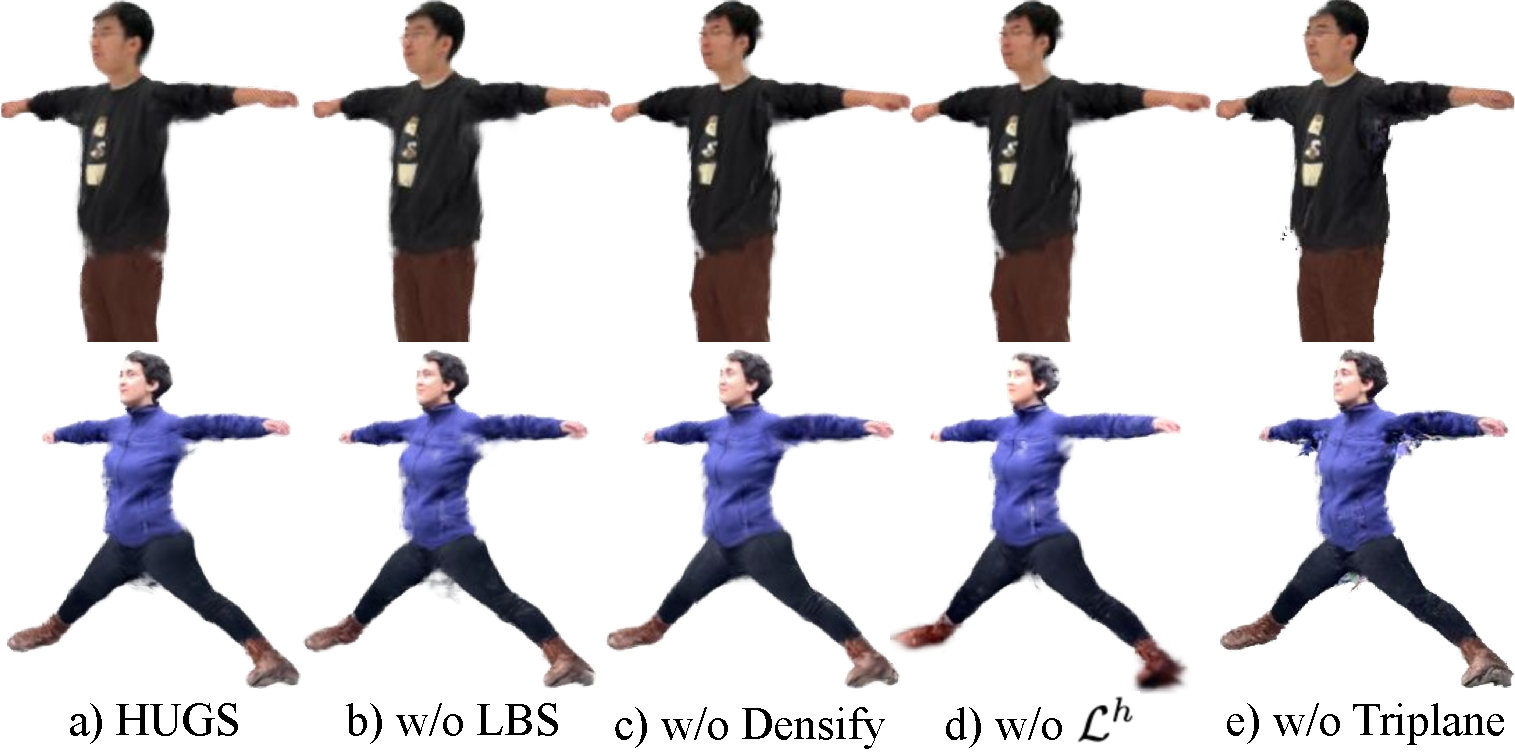
\includegraphics[width=\linewidth]{figures/pdf_files/ablation_qual.pdf}
    % \begin{tabular}{cc}
    %      NeuMan~\cite{jiang2022neuman} \quad \quad & \qquad \qquad HUGS (ours) 
    % \end{tabular}
    \caption{\textbf{Ablation study} showing the visualization of details captured in the human canonical shape under different ablations of our method.} 
    \label{fig:ablation}
\end{figure}

We show the effect of ablating over our method in ~\cref{fig:ablation}. We note that removing LBS from our full model results in floating artifacts that are mainly introduced in the corner region or the body. We also experiment by keeping the number of Human Gaussians to be fixed by disabling densification. This results in floaters around the edges (row 1, on the side of the shirt) since noisy Gaussians are not culled and large Gaussians are not split. 

Furthermore, we examine the effect of removing the loss on the human pixels $\mathcal{L}_h$. This results in loss of fine details in the human region as evident from the reconstruction of the shoes (row 2). In addition, removing the triplane+MLP and directly optimizing the 3DGS parameters results in noisy estimates. Please refer to supplemental material for a detailed ablation and analysis of our contributions.

In ~\cref{tab:neuman_ablation_human_only}, we show quantitative results on the NeuMan dataset by evaluating over only the human-regions by cropping it using a tight bounding box. We evaluate rendering quality using PSNR, SSIM and LPIPS metrics.

%In Table~\cref{tab:neuman_ablation}, we conduct ablation experiments to assess the impact of individual components in our method. When the GCN models are removed, and optimization is performed directly on the 3D Gaussian parameters, the resulting surfaces exhibit increased noise and incompleteness.

% \ar{left $\downarrow$ for MK's reference}

% Ablation experiments will include these discussions:
% \begin{itemize}
%     \item Discuss the effect of replacing GCN with MLP.
%     \item Discuss removing LBS and Posedirs and using SMPL LBS + Posedirs
%     \item Discuss the effect of normal and scale regularizers
%     \item Discuss the effect of joint scene\&human optimization vs. separate optimization
% \end{itemize}

% \subsection{Demos}

% \paragraph{Benefits of using SMPL topology} Leveraging SMPL as the template provides several advantages. It enables the manipulation of body shape using SMPL shape parameters. Also using the consistent SMPL topology allows us to transfer properties from one subject to another \eg clothing. Most significantly, the deformation parameters of SMPL serve as effective regularization for the estimated LBS and pose correctives.

% Since our representation is explicit, we can even simulate the human body in a physical simulation

% \textcolor{red}{MK: mention that triplane results in much lower number of gaussians compared to wo Triplane version}

% \begin{figure*}[t]
    \centering
    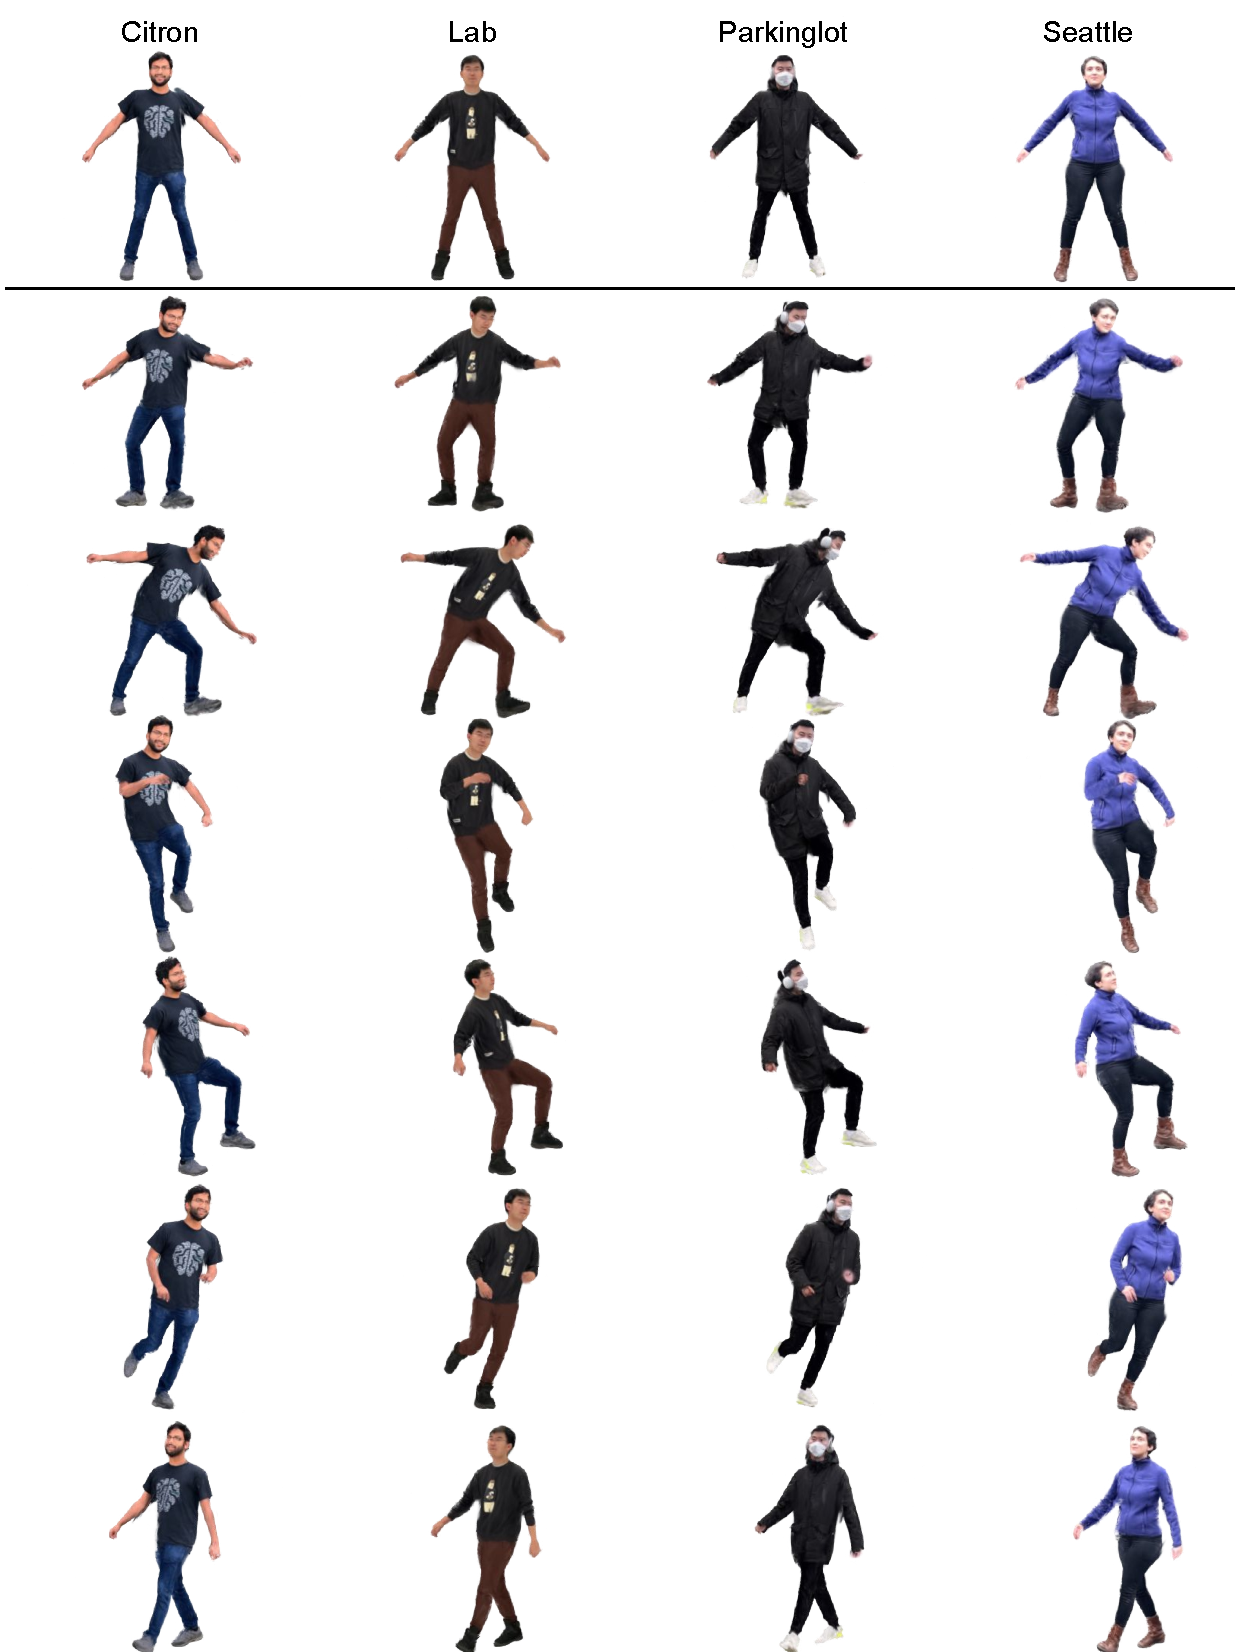
\includegraphics[width=0.9\linewidth]{figures/pdf_files/posed_imgs.pdf}
    \caption{\textbf{Novel pose renderings} We demonstrate the novel pose renderings of subjects (top row) from the NeuMan dataset.} 
    \label{fig:posed_renders}
\end{figure*}{}
% % \begin{figure*}[t]
%     \centering
%     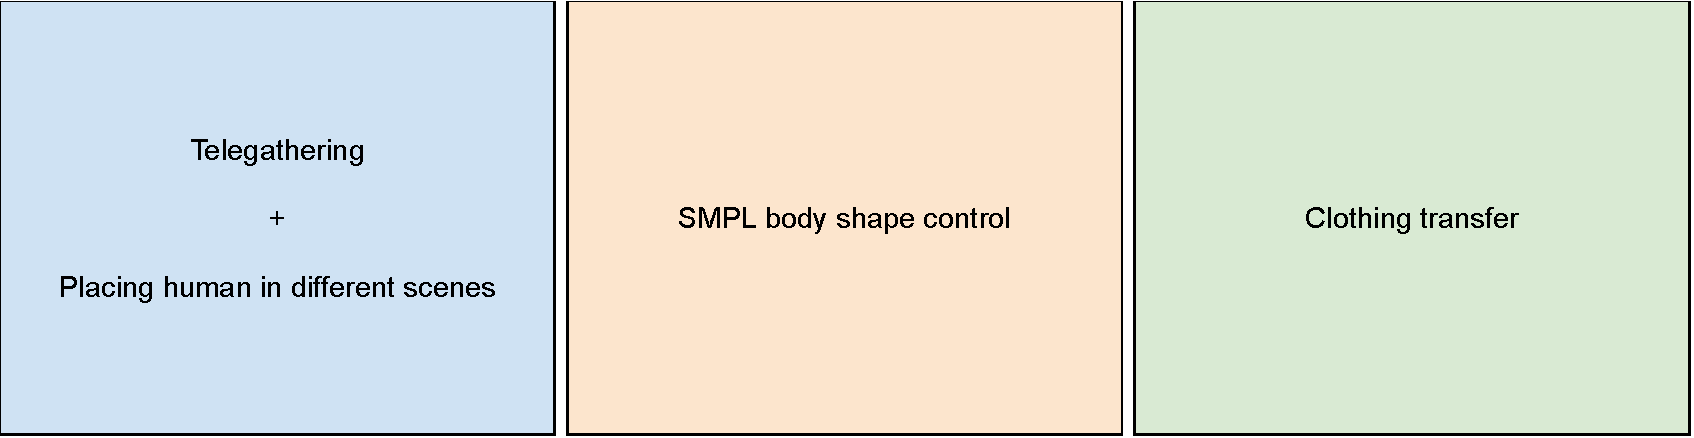
\includegraphics[width=\linewidth]{figures/pdf_files/qual_demo.pdf}
%     \caption{Canonical pose left, novel view animation right} 
%     \label{fig:qual_demo}
%     \vspace{-2ex}
% \end{figure*}{}

